\documentclass{article}
\usepackage{graphicx} % Required for inserting images
\usepackage{hyperref} % Required for links
\usepackage{listings}
\graphicspath{ {./IMG/} }

\title{CAOS-PRJ-WIN-QEMU}
\author{Luca Ponzo}
\date{December 2023}
\begin{document}

\maketitle

\section{Introduction}

In the upcoming steps, this guide will walk you through setting up \textbf{FreeRTOS} and \textbf{QEMU} on Windows. You'll also run a simple demo to make sure everything is working smoothly. To proceed with the installation, keep in mind that there are different choices for an \textbf{SoC} to emulate; in this guide it is used a \textbf{mps-an385}, meaning that it will be explained how to set up an ARM debugger. If you want to install FreeRTOS and QEMU but decide to go with another architecture, please refer to \href{https://www.freertos.org/a00090.html}{the official FreeRTOS documentation}.

\section{QEMU}

To download QEMU on Windows, refer to the official QEMU documentation and download the appropriate executable for your OS architecture, either \href{https://qemu.weilnetz.de/w64/}{64 bit} or \href{https://qemu.weilnetz.de/w32/}{32bit}. After that, open the executable. If it opens just skip chapter \textbf{2.1} (Command prompt execution) and go to \textbf{2.2} (Standard execution).

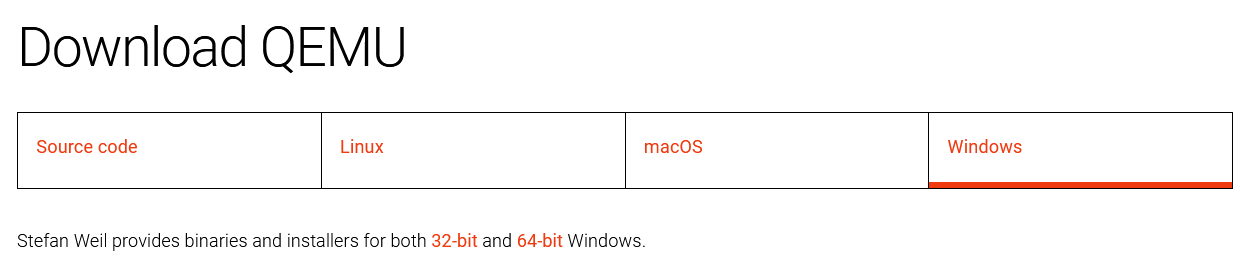
\includegraphics[width=\textwidth]{1a}

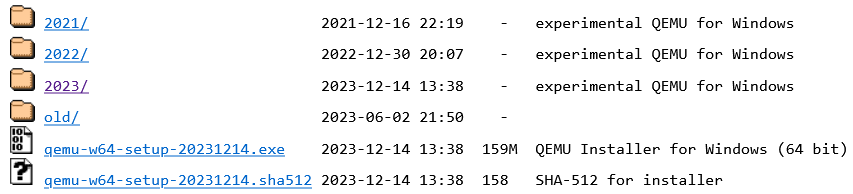
\includegraphics[width=\textwidth]{1b}

\subsection {Command prompt execution}
\begin{enumerate}
    \item Open the command prompt as an administrator
    \item Go to the directory where you saved the QEMU installer
    \item Type the name of the QEMU installer in the command prompt; it should open now
    \item Go forward with the \textbf{Standard installation}.
\end{enumerate}

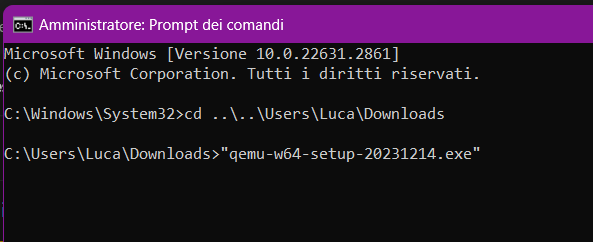
\includegraphics[width=\textwidth]{1c}

\subsection{Standard execution}

Just press forward when it asks and keep in mind the location in which you decide to install QEMU; it will become handy soon.

\subsection {Add to environment path}
After the installation it's needed to add QEMU to the system PATH; you can do it by searching "environment variables" in the Windows Search bar and clicking on the first result. When the window opens:

\begin{enumerate}
    \item Search the item with the text PATH in the upper section of the window
    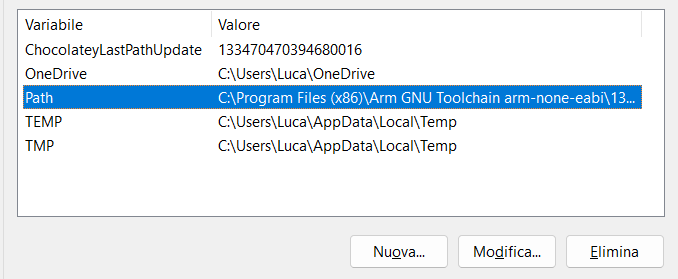
\includegraphics[width=\textwidth]{1d}
    \item Click on edit
    \item Add a new entry and put the path where QEMU is installed (default is \textbf{C:\textbackslash Program Files\textbackslash qemu})

    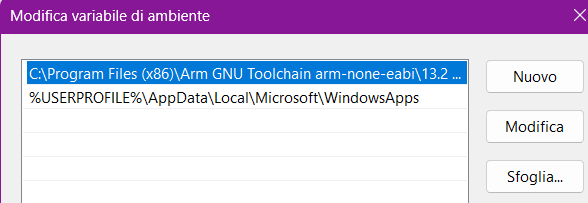
\includegraphics[width=\textwidth]{1e}
    \item Click OK on all the windows opened.
\end{enumerate}

\section{MAKE}

Following the installation of QEMU, additional tools are required to build our FreeRTOS instance. This guide utilizes the \textbf{make} tool, which can be obtained \href{https://gnuwin32.sourceforge.net/packages/make.htms}{from the provided source} Upon selecting the appropriate operating system, you may proceed to initiate the download.

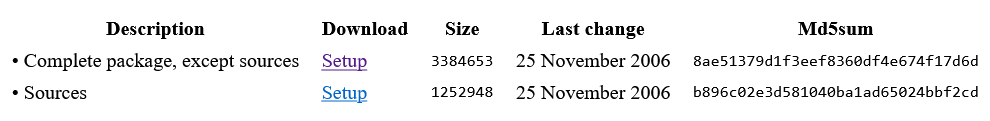
\includegraphics[width=\textwidth]{2a}

\subsection{Installation}
\begin{enumerate}
    \item For the installation process you can just keep pressing forward; the only thing to remember is that you need to \textbf{save the installation path}
    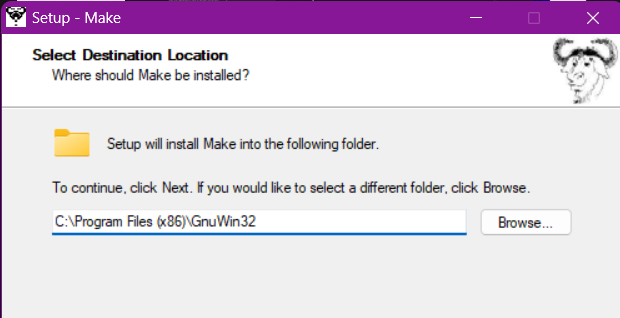
\includegraphics[width=\textwidth]{2b}
    \item After the installation is concluded, add make to the system PATH. Just follow point \textbf{2.3} but change the directory to add from \textit{C:\textbackslash Program Files\textbackslash qemu} to \textbf{make-dir}\textbackslash bin. As an example, if you install make in the same path as the image above, you'll need to add to the environment PATH the directory \textbf{C:\textbackslash Program Files(x86)\textbackslash GnuWin32\textbackslash bin}
    \item Check that make is properly installed by typing \textbf{make -v} in a command prompt window \textbf{freshly opened}. If the prompt gives an error, make sure the PATH you set is correct and then try again.
\end{enumerate}

\section{ARM Toolchain}

Since we are using an ARM SoC, we'll need a matching compiler and debugger. We can download them from \href{https://developer.arm.com/downloads/-/arm-gnu-toolchain-downloads}{the official website}.

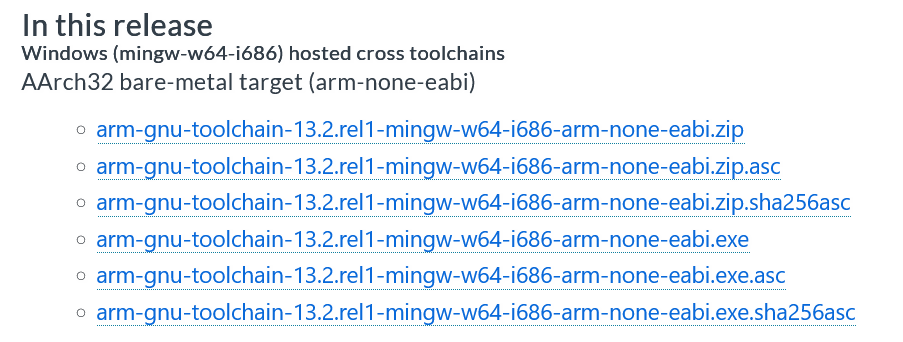
\includegraphics[width=\textwidth]{3a}

\subsection{Installation}
As for the ARM toolchain, life is easier: just make sure to check the box \textbf{Add path to environment variable} in the end. If you didn't, you'll need to refer again to \textbf{2.3} and add \textit{arm-toolchain-dir}\textbackslash bin to the PATH manually.

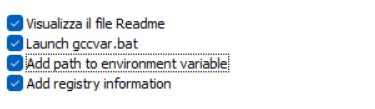
\includegraphics[width=\textwidth]{3b}

\section{FreeRTOS}

Having successfully installed all requisite tools, the next step involves downloading and installing FreeRTOS. As a preliminary measure, it is imperative to initiate the download of the system; in this instance, the process is marginally more intricate than previously described.

\subsection{Download}
\begin{enumerate}
    \item Open a command prompt and navigate to the directory where you intend to store the FreeRTOS files. From now on we'll refer to that directory by \textbf{FreeRTOS-dir}
    \item Enable git's submodules by typing \begin{verbatim}git config --global core.symlinks true\end{verbatim}
    \item Clone the repository by typing \begin{verbatim}git clone https://github.com/FreeRTOS/FreeRTOS.git --recurse-submodules\end{verbatim}
\end{enumerate}

\subsection{Installation}
\begin{enumerate}
    \item Go to \textbf{\textit{FreeRTOS-dir}\textbackslash FreeRTOS\textbackslash Demo\textbackslash CORTEX\textunderscore MPS2\textunderscore QEMU\textunderscore IAR\textunderscore GCC\textbackslash build\textbackslash gcc}
    \item Type \textbf{make}
    \item If all the steps above went fine, you should have the file \textbf{.\textbackslash output\textbackslash RTOSDemo.out}
    \item If you want to run the blink demo, edit \textbf{.\textbackslash output\textbackslash main.o} and make sure the line \textbf{mainCREATE\textunderscore SIMPLE\textunderscore BLINKY\textunderscore DEMO\textunderscore ONLY} is defined to \textbf{1}.

    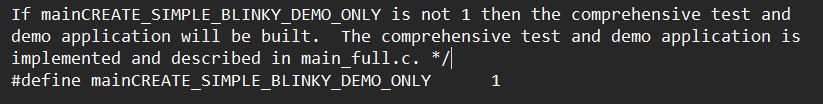
\includegraphics[width=\textwidth]{4}
\end{enumerate}

\subsection{Starting FreeRTOS}
If the installation procedure is concluded, you should be able to run FreeRTOS in QEMU by just typing one single command:
\begin{verbatim}
qemu-system-arm -machine mps2-an385 -cpu cortex-m3 -kernel
<FreeRTOS-dir>\FreeRTOS\Demo\CORTEX_MPS2_QEMU_IAR_GCC\build\gcc\output\RTOSDemo.out
-monitor stdio -s -S
\end{verbatim}

\subsection{Debugger utilization}
\begin{enumerate}
    \item Open a new command prompt and go to the directory of RTOSDemo.out
    \item Type the command \begin{verbatim}
        arm-none-eabi-gdb RTOSDemo.out
    \end{verbatim}
    \item Connect to the QEMU instance; it should be opened in the default port: \textbf{1234}. You can do that by typing \begin{verbatim}
        target remote localhost:1234
    \end{verbatim}
    \item If you type \textbf{continue}, the blinky demo will start.
\end{enumerate}

\end{document}
